\subsection{Desarrollo y verificación de módulos comunes}
Se comenzo describiendo en Verilog los módulos comunes que serán utilizados posteriormente como parte de los bloques correspondientes al encoder y al decoder. 

Una vez implementados, los módulos fueron verificados mediante un testbench sencillo en UVM, con secuencias básicas para validar el funcionamiento de cada uno.

\subsection{Analisis: Posible modificacion del decoder}
Para el decoder la arquitectura propuesta plantea el cálculo del síndrome y del vector $q$ en etapas diferentes del pipeline. A partir de las propiedades del código, en particular de la condición $B^2 = I$, se analizó una posible modificación de la arquitectura en la cual se calculan el syndrome y $q$ en la primera  tapa del pipeline directamente usando el vector recibido $r$.\\

Considerando al vector $r$ por sus componentes $r_h$ (alta) y $r_l$ (baja), y como el síndrome:
\begin{align*}
    s = r_h \cdot B + r_l
\end{align*}

Como el vector $q$ se obtiene a partir del síndrome, si aprovechamos la propiedad $B^2 = I$ se puede expresar $q$ directamente en
función de los componentes del vector recibido:
\begin{align*}
    q &= s\cdot B \\
    &= (r_h\cdot B + r_l)\cdot B\\
    &= r_h\cdot B^2 + r_l\cdot B \\
    &= r_h\cdot I + r_l\cdot B \\
    &= r_h + r_l\cdot B
\end{align*}

De esta manera se permite plantear una alternativa donde el síndrome y el vector $q$ serían calculados a partir de $r$ durante la primera etapa del pipeline.\\

Sin embargo, el análisis de la implementación mostró que la modificación requiere una cantidad adicional de lógica que no resultaba conveniente para la arquitectura propuesta. En particular, se agregan 12 compuertas XOR adicionales, junto con la lógica necesaria para seleccionar el cálculo correspondiente al síndrome o al vector $q$.\\

Considerando tanto el incremento logica como un analisis basico de la actividad de switching de los modulos cuando cambia el vector r, se descartó esta alternativa. Por lo tanto, se mantuvo la arquitectura originalmente propuesta, conservando el cálculo del síndrome y del vector $q$ en las etapas de pipeline inicialmente definidas.

\subsection{Implementación RTL del encoder}
(Parte de AbeliyoPiyo vvvvvv)
* RTL DEL ENCODER

\subsection{Resumen del encoder}
\begin{figure}[H]
    \centering
    \includegraphics[scale=0.3]{encoder-theros1.png}
    % \caption{Implementación RTL del encoder.}
    \label{fig:encoder-theros1}
\end{figure}

\begin{figure}[H]
    \centering
    \includegraphics[scale=0.3]{encoder-theros2.png}
    \caption{Resumen de la implementación RTL del encoder.}
    \label{fig:encoder-theros2}
\end{figure}

\subsection{Implementación RTL del decoder}

A partir de los módulos comunes, se describieron bloques para el cálculo del síndrome, del vector $q$, la búsqueda por filas y la generacion de la máscara de error mediante los diferentes casos en la decodificación.

Cada uno fue validado mediante el testbench UVM, utilizando secuencias de estímulos basicas para verificar su funcionamiento.\\

Una vez validados los módulos, se incorporaron los registros de pipeline correspondientes para integrar el top del decoder. Quedando la arquitectura final y cada etapa logica:

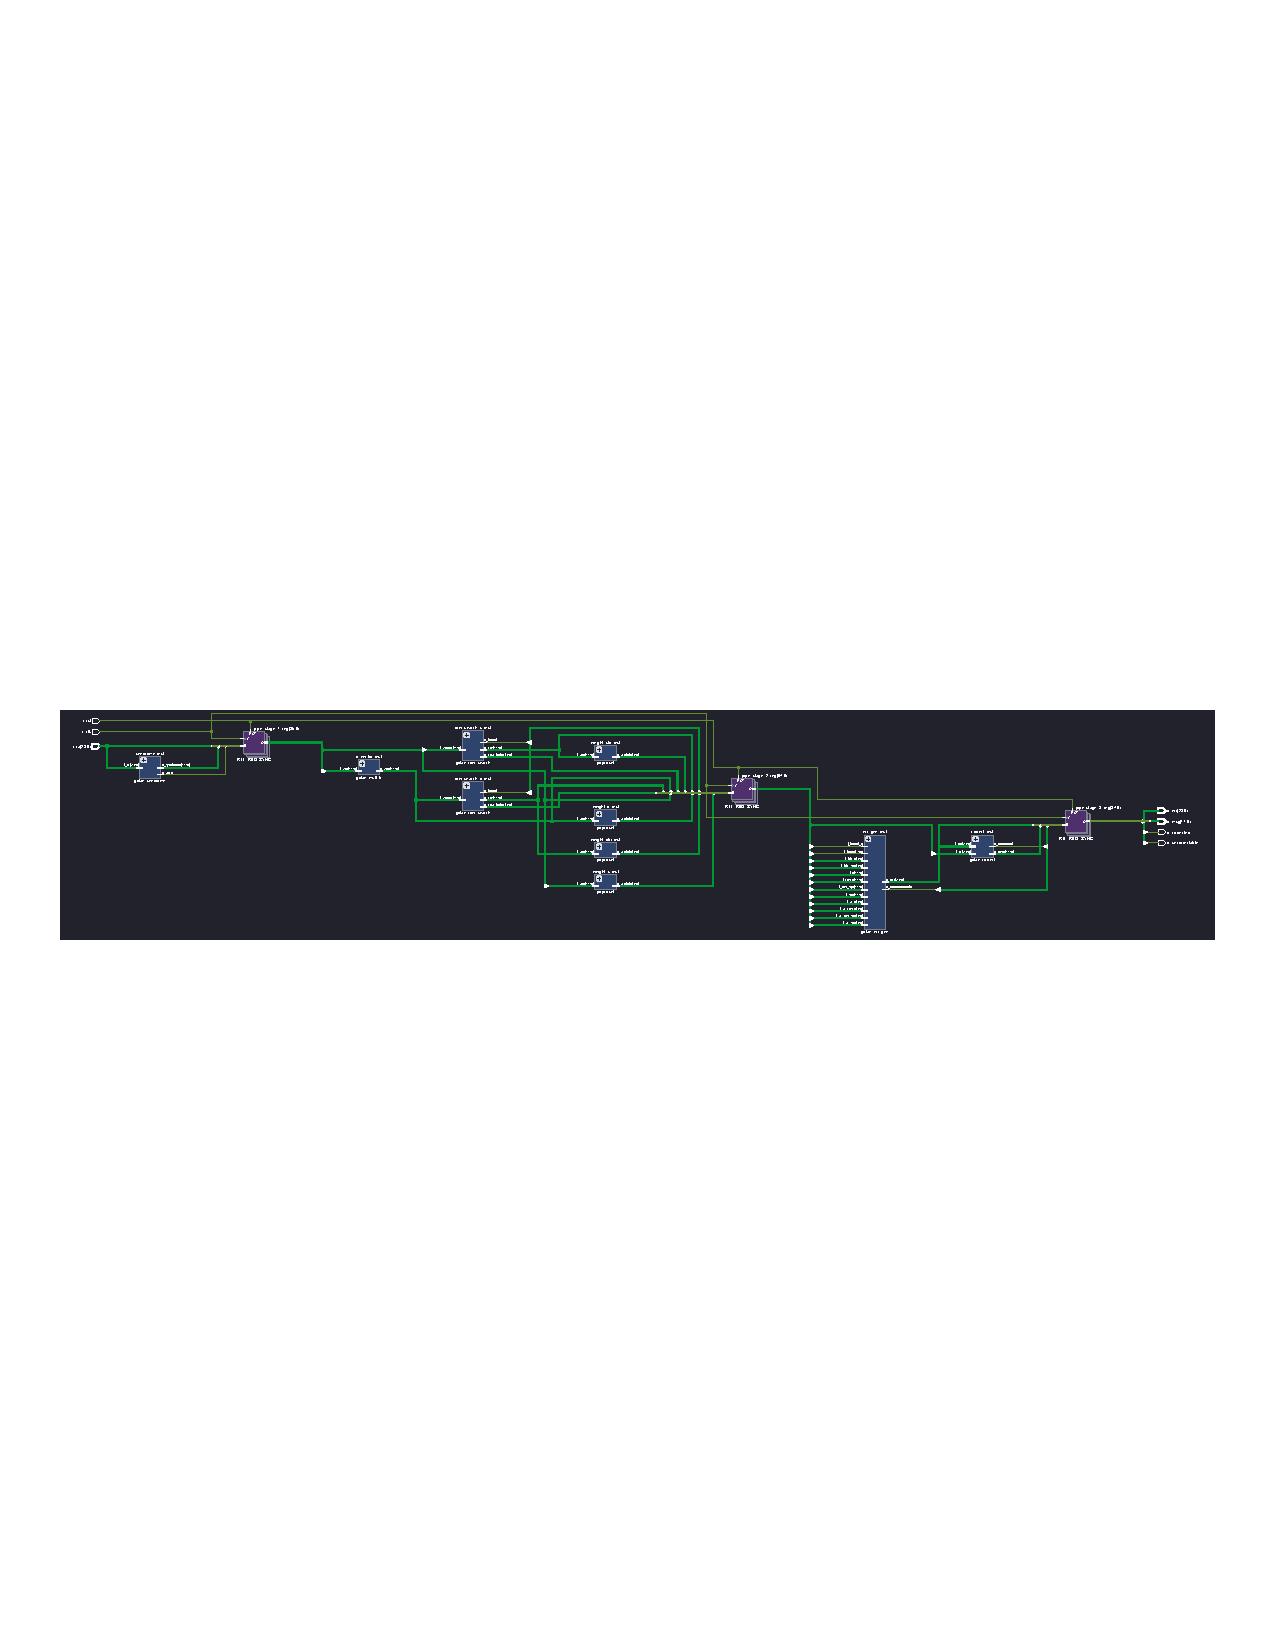
\includepdf[pages=-]{inc/decoder.pdf}

\begin{figure}[H]
    \centering
    \includegraphics[scale=0.25]{decoder-stage1.png}
    \caption{Primera etapa del pipeline del decoder.}
    \label{fig:decoder-stage1}
\end{figure}

\begin{figure}[H]
    \centering
    \includegraphics[scale=0.25]{decoder-stage2.png}
    \caption{Segunda etapa del pipeline del decoder.}
    \label{fig:decoder-stage2}
\end{figure}

\begin{figure}[H]
    \centering
    \includegraphics[scale=0.25]{decoder-stage3.png}
    \caption{Tercera etapa del pipeline del decoder.}
    \label{fig:decoder-stage3}
\end{figure}

\subsection{Resumen del decoder}
\begin{figure}[H]
    \centering
    \includegraphics[scale=0.3]{decoder-theros1.png}
    % \caption{Implementación RTL del decoder.}
    \label{fig:decoder-theros1}
\end{figure}

\begin{figure}[H]
    \centering
    \includegraphics[scale=0.3]{decoder-theros2.png}
    \caption{Resumen de la implementación RTL del decoder.}
    \label{fig:decoder-theros2}
\end{figure}

\subsection{Validacion del decoder}
Se realizó su verificación funcional usando el entorno UVM mediante vector matching, con archivos de referencia generados a partir del modelo desarrollado previamente. En los vectores cada línea contiene el vector de entrada $rx$ y las salidas esperadas correspondientes al mensaje decodificado, el patrón de error y las flags corrected y uncorrectable.\\

Como primera verificación funcional, se utilizaron codewords sin errores. En este caso se verificó que el patrón de error sea nulo, y que las señales corrected y uncorrectable permanecieran en bajo durante todo el test. La Figura~\ref{fig:decoder-wave-codeword-only} muestra los resultados obtenidos durante el test:

\begin{figure}[H]
    \centering
    \includegraphics[scale=0.32]{decoder-wave-codeword-only.png}
    \caption{Verificación del decoder utilizando codewords sin errores.}
    \label{fig:decoder-wave-codeword-only}
\end{figure}

En esta ventana se observa tambien la latencia de tres ciclos esperada. Sobre el primer cursor, en hexadecimal los tres dígitos superiores de rx corresponden al mensaje 001h junto con los bits de paridad correspondientes EA9h. Luego de tres ciclos, se obtiene a la salida el mismo mensaje decodificado.

\subsection{Correcciónes en el decoder}
A continuación, se realizó una segunda prueba aplicando en cada codeword todos los patrones de error posibles correspondientes a pesos de error entre cero y cuatro.\\

Durante la verificación se detectaron algunos errores en el
decoder. Los problemas estuvieron relacionados a condiciones en la generación de la máscara de error y al conexionado entre
los diferentes módulos.

Por observacion y analisis, se identificaron los problemas y se realizaron las
correcciones correspondientes. Luego de aplicar las correcciones, se logró validar el funcionamiento del
decoder para los casos contemplados en el test.\\

Se puede ver un waveform general del test donde, muy resumidamente, luego de salir del reset se aplican errores de peso 0 a 3 donde se recupera el mensaje original (EFEh) y se reporta los casos como corrected. Luego se insertan errores de peso 4 hasta el final del test y se reportan como uncorrectable:

\begin{figure}[H]
    \centering
    \includegraphics[scale=0.25]{decoder-wave-full.png}
    \caption{Simulación del decoder para los patrones de error evaluados.}
    \label{fig:decoder-wave-full}
\end{figure}

Y tambien se agrego un objeto en el testbench para reportar la cantidad de patrones de error por peso (en formato de array error\_weight[weight]) y la cantidad de casos corregidos y detectados. Se obtuvieron los valores de la tabla verificada en la PARTE B (Ejercicio 7 Caracterización del decodificador): 

\begin{figure}[H]
    \centering
    \includegraphics[scale=0.4]{decoder-error-table.png}
    \caption{Tabla de casos de decodificacion segun peso de error (modelo).}
    \label{fig:decoder-error-table}
\end{figure}

\begin{figure}[H]
    \centering
    \includegraphics[scale=0.3]{report-table.png}
    \caption{Tabla de casos de decodificacion segun peso de error (RTL).}
    \label{fig:decoder-report-table}
\end{figure}

Finalmente, se verificó el funcionamiento del decoder utilizando las
codewords correspondientes a la PARTE A (Ejercicio 3 Decodificación manual). Las tres codewords fueron aplicadas
como vectores de entrada y se verificó su correspondiente decodificación. La
Figura~\ref{fig:decoder-wave-3codeword} muestra las señales obtenidas durante
esta prueba.

\begin{figure}[H]
    \centering
    \includegraphics[scale=0.3]{decoder-wave-3codeword.png}
    \caption{Decodificación de las tres codewords correspondientes a la PARTE A.}
    \label{fig:decoder-wave-3codeword}
\end{figure}

\subsection{Integración del top level}
En esta etapa se realizó la integración de los módulos desarrollados
previamente obteniendo el top level del diseño. Para ello, se
instanciaron los módulos encoder, decoder e inyector de
errores, estableciendo las conexiones necesarias entre ellos de acuerdo con
la arquitectura definida.

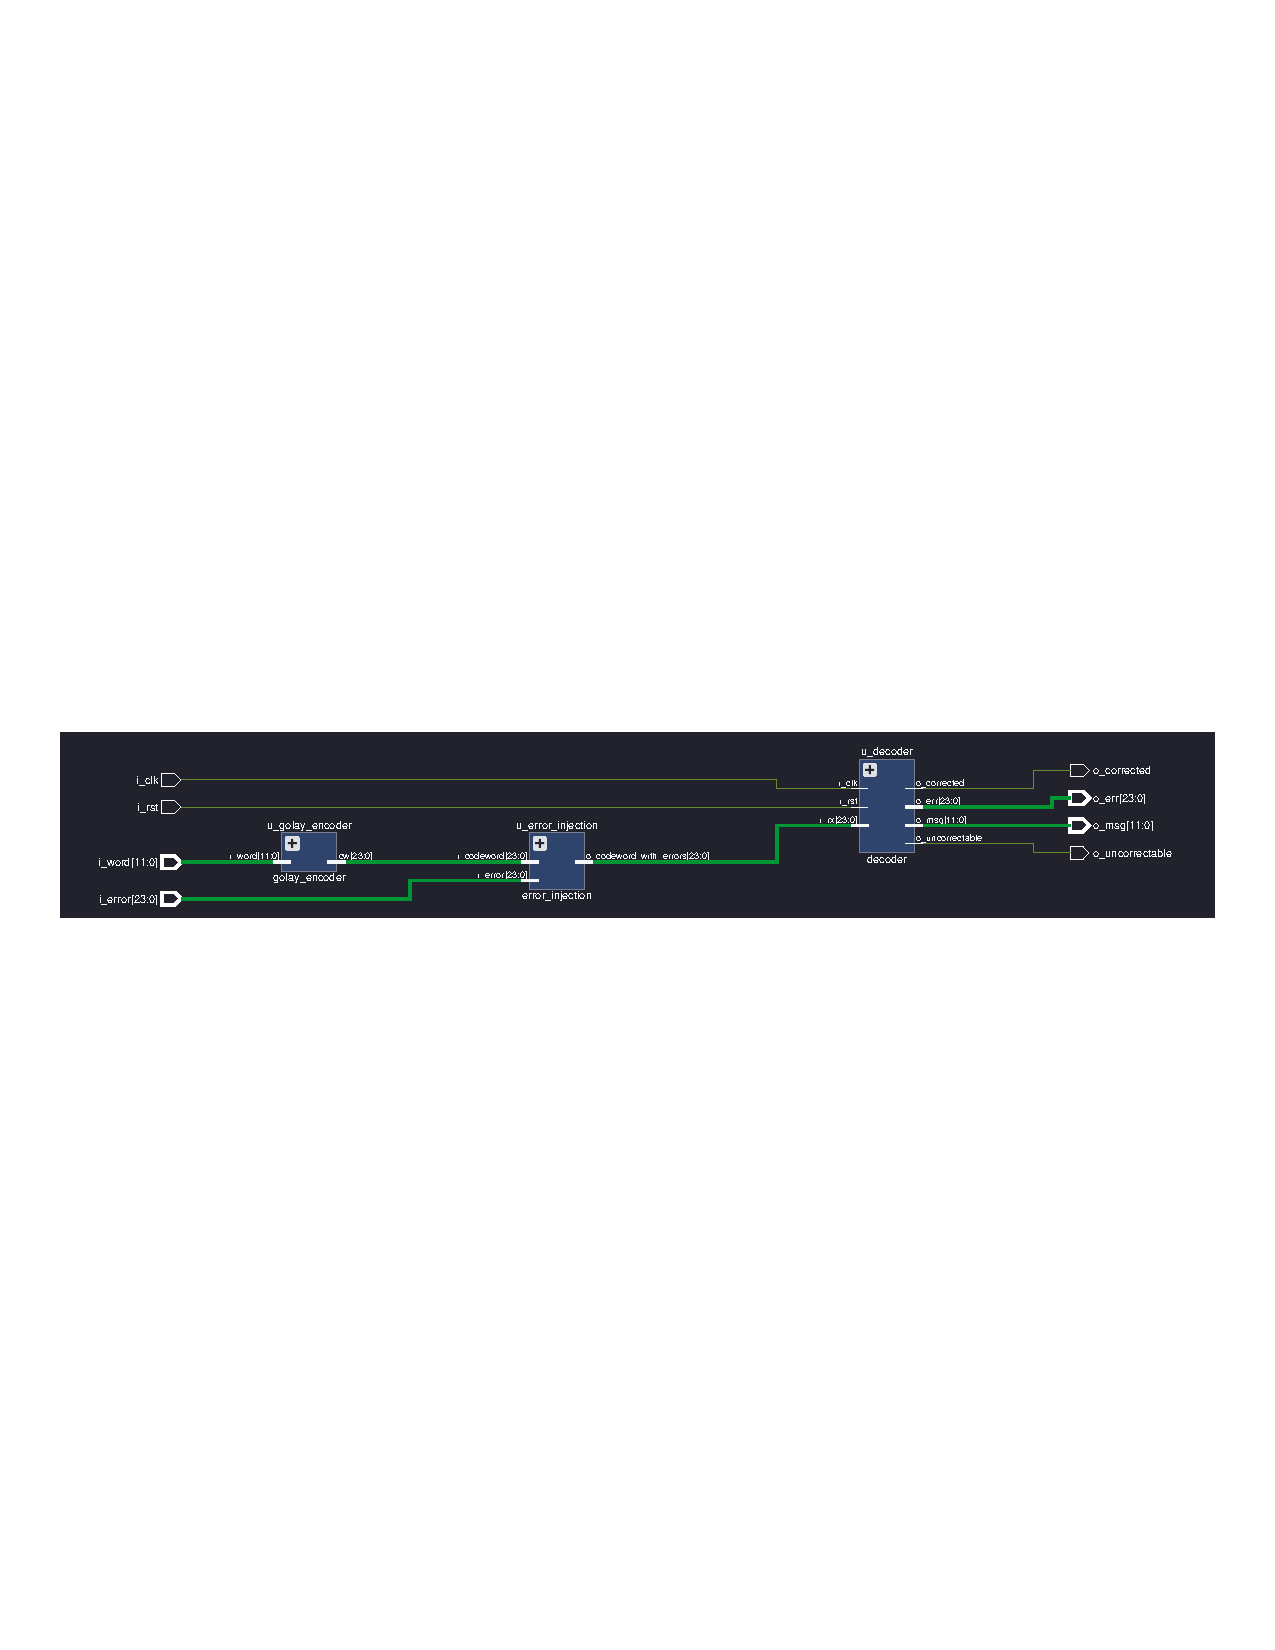
\includepdf[pages=-]{inc/top.pdf}

\subsection{Verificación del top level}

Una vez integrado el top level, se generaron los vectores necesarios para
validar el funcionamiento de la arquitectura final. Cada línea del archivo
de vectores contiene, en orden, la palabra a transmitir y el patrón de error
a aplicar. Como resultados esperados se incluyen el mensaje decodificado, la
máscara de error detectada y las señales corrected y uncorrectable.

La validación se realizó mediante el entorno UVM,
utilizando vector matching entre los resultados obtenidos por el diseño RTL
y los valores generados previamente a partir del modelo de referencia. La
Figura~\ref{fig:top-wave-general} muestra una vista general de la simulación
correspondiente al test, donde se aplican patrones de error de peso
menor o igual a tres, seguida por una región en la que se aplican patrones de
error incorregibles.

\begin{figure}[H]
    \centering
    \includegraphics[scale=0.3]{top-wave-general.png}
    \caption{Waveform general correspondiente a la verificación del top level.}
    \label{fig:top-wave-general}
\end{figure}

Al salir del reset se aplica la palabra EFEh sin ningún
patrón de error, luego de tres ciclos se obtiene el mensaje decodificado y el patrón de error detectado es
nulo. Este comportamiento se muestra en la
Figura~\ref{fig:top-wave-error-w0}.

\begin{figure}[H]
    \centering
    \includegraphics[scale=0.34]{top-wave-error-w0.png}
    \caption{Decodificación sin errores y verificación de la latencia.}
    \label{fig:top-wave-error-w0}
\end{figure}

A continuación, se incrementó el peso del patrón de error aplicado. En la
Figura~\ref{fig:top-wave-error-w1w2} se muestra la transición desde un patrón
de error de peso uno hacia uno de peso dos.

\begin{figure}[H]
    \centering
    \includegraphics[scale=0.36]{top-wave-error-w1w2.png}
    \caption{Transición entre patrones de error de peso uno y dos.}
    \label{fig:top-wave-error-w1w2}
\end{figure}

La Figura~\ref{fig:top-wave-error-w2w3} muestra la transición desde un patrón
de error de peso dos hacia uno de peso tres.

\begin{figure}[H]
    \centering
    \includegraphics[scale=0.34]{top-wave-error-w2w3.png}
    \caption{Transición entre patrones de error de peso dos y tres.}
    \label{fig:top-wave-error-w2w3}
\end{figure}

Finalmente, en la Figura~\ref{fig:top-wave-error-w3w4} se observa la
transición hacia un patrón de error de peso cuatro. A partir de este punto,
la señal uncorrectable permanece en alto, indicando que el patrón de error
aplicado no puede ser corregido por el decoder. En esta condición, las
salidas correspondientes al mensaje y al patrón de error detectado se
consideran inválidas.

\begin{figure}[H]
    \centering
    \includegraphics[scale=0.33]{top-wave-error-w3w4.png}
    \caption{Transición entre patrones de error corregibles e incorregibles.}
    \label{fig:top-wave-error-w3w4}
\end{figure}

